\section{Entwickeln der 2D-DFT in VHDL}

Ziel ist es die gleiche DFT-Einheit für beide DFTs zu verwenden

Zähler für 64 Werte kann als 6 Bit Vektor realisiert werden, der bei 63 einen Überlauf hat und wieder bei 0 anfängt.

Vorderen 3 Bit sind die der Zeile, die hinteren für die Spalte.

Das dritte Bit von vorne sagt einem, ob es eine gerade oder ungerade Zeile ist.


 
 
 
Die in Gleichung (\ref{eq:2D-DFT_MatrixMult}) beschriebene Berechnung der 2D-DFT lässt sich auch wie folgt schreiben:

\begin{align}
 X &= W \cdot x \cdot W \nonumber \\
   &= \left(x^T\cdot W\right)^T\cdot W \label{eq:MatMultTranspose1} \\
   &= X^* \cdot W \nonumber\\
   &= \left(\left(x\cdot W\right)^T\cdot W\right)^T \label{eq:MatMultTranspose2}\\
   &= \left(X^{*T} \cdot W\right)^T \nonumber
\end{align}

In Matlab muss hierfür entweder die Funktion \texttt{transpose()} oder \texttt{.'} verwendet werden. Letzteres muss elementweise angewandt werden, da das Apostroph
alleine die komplex konjugiert Transponierte bildet.

Die alternativen Schreibweisen der 2D-DFT haben den Vorteil, dass in beiden Fällen die Eingangsmatrix auf der linken Seite steht. Möglich ist dies, da die 
Twiddlefaktormatrix identisch mit ihrer Transponierten ist.
Dass nun in den Gleichungen (\ref{eq:MatMultTranspose1}) und (\ref{eq:MatMultTranspose2}) sowohl die Eingangs- als auch die 1D-DFT-Matrix links steht, ist eine wichtige 
Voraussetzung dafür, dass mit der selben Recheneinheit mit der die 1D-DFT berechnet wird auch die 2D-DFT berechnet werden kann.
Die zweite Voraussetzung ist das Transponieren einer Matrix. Diese lässt sich durch spaltenweises Abspeichern und zeilenweises Auslesen der Ergebnis-Matrix realisieren.
Hierfür ist es lediglich notwendig die beiden Indizes, welche ein Matrixelement ansprechen, beim Speichern getauscht werden. Nun sind nun alle Voraussetzungen erfüllt, 
um beide Berechnungen mit der selben Einheit durch zu führen. In Grafik (\ref{pic:MatMultTranspose}) ist das hier beschriebene veranschaulicht.

(Auf diese Weise wird die direkte Weiterverarbeitung von Werten denkbar.)
 
\begin{figure}[htbp]
 \centering
 \includegraphics[width=0.95\textwidth]{img/MatMultTranspose2.png}
 \caption{Darstellung der Berechnung der 2D-DFT aus Gleichung (\ref{eq:MatMultTranspose2})}
 \label{pic:MatMultTranspose}
\end{figure}
 

\section{Direkte Weiterverarbeitung der Zwischenergebnisse}
Um die Anzahl an Gattern und somit den Flächenbedarf zu reduzieren ist es das Ziel, die Ergebnisse der \gls{1d-dft} aus der 1. Berechnungsstufe im nächsten Schritt direkt als 
Eingangswerte für die \gls{2d-dft} zu verwenden. Auf diese Weise würden 64$\cdot$2$\cdot$12 Bit = 1536 Bit = 1,5kBit = 192 Byte an Speicher eingespart werden.
Wie sich im Laufe der Entwicklung gezeigt hat, lässt sich das nicht nutzen. Das liegt daran, dass dazu übergegangen wurde, immer nur ein Element zur Zeit berechnet wird und die 
bereits errechneten demnach zwischengespeichert werden müssen. Dieser Ansatz wurde verfolgt, da der Entwicklungsaufwand in VHDL für die spaltenweise Berechnung der Ausgangswerte 
einfacher umzusetzen war und es zunächst nur um die mathematische Umsetzung und nicht um die Platzeffizienz auf einem Chip ging.

Unklar war zu diesem Zeitpunkt noch, wie der Speicher realisiert werden soll. In der finalen Variante des Chips soll es einen \gls{ram} geben, der als zentraler
Speicher von allen Komponenten genutzt wird. Da die Entwicklung im Projekt noch nicht soweit fortgeschritten ist und dies nicht zu den Aufgaben der vorliegenden Arbeit gehört,
wurde auf das Speichern in lokalen Speicherzellen ausgewichen, welche als Variable oder Signal im VHDL-Code definiert und von der Software als Flip-Flop synthetisiert werden.



%\section{Umsetzung der Optimierungen}
\section{Optimierte 8x8 DFT als Matrixmultiplikation}\label{sec:OptimierteMatrixmultiplikation}
Anfangs wurde in Betracht gezogen das 1er-Komplement zu verwenden, da hierbei zwei betragsmäßig identische Zahen sich nur durch ihr höchstwertigstes 
 Bit unterscheiden. Auf diese Weise könnte das selbe Resultat für den Imaginär- wie für den Realteil verwendet werden, das Vorzeichen würde sich über eine 
 einfache XOR-Verknüpfung beider MSB der Multiplikanden ergeben.
 Diesem Vorteil steht jedoch eine aufwändigere Subtraktion (bzw. Addition negativer Zahlen) gegenüber. Der zusätzliche Aufwand entspricht 
 etwa dem der Bildung des 2er-Komplements. Aus diesem Grund und da das 2er-Komplement deutlich verbreiteter ist sowie weitere Vorteile bringt wie 
 beispielsweise keine Doppeldeutigkeit durch eine negative Null hat, wurde sich hierfür entschieden.
 
 
 In späteren Analysen konnte festgestellt werden, dass sowohl für den Real- als auch den Imaginärteil gleichviele Multiplikationen mit positiven wie mit negativen Faktoren 
 durchgefürht werden müssen. Dies lässt sich anhand des Einheitskreises in Abb. \ref{pic:Einheitskreis_Faktoren} und der Abbildung \ref{pic:Twiddlefaktoren_Darstellung8x8}
 nachvollziehen. Aus Abschnitt \ref{sec:Matrixmultiplikation} ist bekannt, dass bei einer Matrixmultiplikation Elemente multipliziert und anschließend die Ergebnisse 
 aufsummiert. Da es das Kommutativgesetz erlaubt die berechneten Ergebnisse auch in einer anderen Reihenfolge zu addieren, 

 
   
 In Abbildung \ref{pic:MatrizenDarstellungTwiddlefaktoren} ist zu sehen, dass die 2., 4., 6., und 8. Zeile je vier nicht triviale und komplexe Faktoren enthält. 
 Darüber hinaus ist ersichtlich, dass für komplexe Eingangswerte in den genannten Zeilen 12 und in den übrigen 8 Multiplikationen erfolgen müssen. Dies kann anhand der 
 Gleichungen (\ref{eq:komplexe_Multiplikation}) und (\ref{eq:halb_komplexe_Multiplikation}) nachvollzogen werden.
 Das lässt sich ausnutzen, um keine Negationen der Eingangs- und Zwischenwerte durchführen zu müssen. 
 

 
 Darüber hinaus
 minimiert sich bei geschickter Anordnung das Risiko eines Überlaufs. Wie in Abschnitt \ref{sec:NumerischeUngenauigkeiten} erwähnt, ist dies nicht Gegenstand dieser Arbeit,
 weshalb der Einfachheit wegen zur Sicherheit dennoch nach jeder Addition oder Subtraktion das Ergebnis durch einen Bitshift halbiert wird. 
 Es sei an dieser Stelle lediglich angemerkt, dass über die Eingangswerte die Annahme getroffen werden kann, dass aufeinanderfolgende Werte das selbe Vorzeichen haben. 
 Dies ließe sich ausnutzen, um noch weiter die Wahrscheinlichkeit zu reduzieren, dass es zu einem Überlauf kommt. 
 

 




% Später wohl besser ins Kapitel Entwicklung
Dies hat zur Folge, dass ein sehr großer Wert entstehen kann, welcher Maßgebend für die Anzahl der Vorkommabits sein kann.
%
Wegen der Null im Imaginärteil der ersten Zeile der Twiddlefaktormatrix sind auch alle Imaginärteile der ersten Spalte der Ausgangsmatrix Null.
Bezogen auf den Imaginärteil gilt das Gleiche auch für die fünfte Zeile der Twiddlefaktormatrix. 
%
Da sich beim Realteil der fünften Zeile der Twiddlefaktormatrix der fünften Zeile positive und negative Einsen abwechseln, sind hier auch keinerlei Multiplikationen nötig.

Aus der anfänglichen Implementation bei der alle nicht trivialen Werte einer Berechnung die entweder mit $+\frac{\sqrt{2}}{2}$ oder $-\frac{\sqrt{2}}{2}$ multipliziert wurden,
einzelnd berechnet werden, wird mittels des Distributivgesetzes der gemeinsame Faktor ausgeklammert, sodass nur noch jeweils eine Multiplikation erforderlich ist.


Bei den weiteren Zeilen sind hingegen die Zahlen zur Hälfte positiv und zur anderen negativ. Außerdem enthalten die geraden Zeilen den Faktor $\pm\frac{\sqrt{2}}{2}$. 
Dies lässt sich ausnutzen, um die Anzahl der der Multiplikationen zu reduzieren. Zunächst können die 

Für jede gerade Zeile der DFT ist jeweils für den Real- und den Imaginärteil eine Multiplikation nötig, so dass sich insgesamt acht Multiplikationen ergeben
 
\subsection{W = transpose(W)}
 
 
\section{Berechnungsschema der geraden und ungeraden Zeilen}\label{sec:Berechnungsschema}

In Abbildung \ref{pic:AkkumulationUngeradeSpalten} ist die Berechnung der ungeraden Zeilen am Beispiel der ersten zu sehen.

\begin{figure}[htbp]
\centering
$a_{0} + a_{1} + a_{2} + a_{3} + a_{4} + a_{5} + a_{6} + a_{7}$\\

\vspace{0.5cm}
\begin{tabular}{ccccccccc}
Takt&\multicolumn{6}{l}{ } & & Bit\\
1&$\underbrace{a_{k0} + a_{k1}}$ &  &$ \underbrace{a_{k2} + a_{k3}}$ &  &$\underbrace{a_{k4} + a_{k5}}$ &  &$\underbrace{a_{k6} + a_{k7}}$ & 12\\
&\multicolumn{7}{l}{$\hspace{0.65cm} \Downarrow \hspace{2.3cm} \Downarrow \hspace{2.3cm} \Downarrow \hspace{2.3cm}\Downarrow$}&13\\
2&\multicolumn{3}{c}{$\underbrace{sum\_1\_1 \quad + \quad sum\_1\_2}$} & & \multicolumn{3}{c}{$\underbrace{sum\_1\_3 \quad + \quad sum\_1\_4}$} & 12\\
&\multicolumn{3}{c}{$\Downarrow$} & & \multicolumn{3}{c}{$\Downarrow$}&13\\
3&\multicolumn{7}{c}{$\underbrace{sum\_2\_1 \quad  \quad \quad \quad + \quad \quad \quad  \quad sum\_2\_2}$} & 12\\
&\multicolumn{7}{c}{$\Downarrow$}&13\\
&\multicolumn{7}{c}{$sum\_3\_1$} & 12\\
&\end{tabular}
%\captionof{figure}{Vorgehensweise der Akkumulation der ungeraden Spalten der Eingangswerte}
\caption{Vorgehensweise der Akkumulation der ungeraden Spalten der Eingangswerte.}
\label{pic:AkkumulationUngeradeSpalten}
\end{figure}
%\end{center}

\vspace{0.5cm}

Wie der linken Spalte zu entnehmen ist, werden 3 Takte für die Berechnungen der Werte aus den ungeraden Spalten der Eingangsmatrix bzw. ungeraden Zeilen der 1D-DFT-Matrix benötigt.
1. Takt für Additionen bzw. Subtraktionen und 2. sowie 3. Takt für das Aufsummieren. Der Bitvektor des Ergebnisses ist zwar 12 Bit breit, aber beim letzten Bitshift von 13 auf 12
werden nur 11 Bit übernommen. Es wird alo ein doppelter Bitshift vollzogen. Dies erfolgt, damit sowohl in den geraden als auch den ungeraden Zeilen gleich viele Bitshifts erfolgen
und die Werte somit identisch skaliert sind.

Die Berechnung der geraden Zeilen wird in Abbildung \ref{pic:AkkumulationGeradeSpalten} am Beispiel der zweiten Zeile gezeigt
\begin{figure}[htbp]
 \centering
 $a_0 - x_1 + x_0 - b_2 + x_2 - x_3 + a_4 - x_5 + x_4 - b_6 + x_6 - x_7$\\

 \vspace{0.3cm}
 
\begin{tabular}{ccccccccccccc}
Takt&\multicolumn{11}{c}{}&Bit\\
1 &$\underbrace{a_0 - x_1}$ &        &$ \underbrace{x_0 - b_2}$ &  &$\underbrace{x_2 - x_3}$ &  &$\underbrace{a_4 - x_5}$ &  &$\underbrace{x_4 - b_6}$ &$\underbrace{x_6 - x_7}$& &12\\
  &\multicolumn{11}{l}{$\hspace{0.5cm} \Downarrow \hspace{1.75cm} \Downarrow \hspace{2.4cm} \Downarrow \hspace{1.8cm}\Downarrow \hspace{1.8cm}\Downarrow \hspace{1.4cm}\Downarrow$}&13\\
2 &\multicolumn{3}{c}{$\underbrace{sum1\_1 \: + \: sum1\_2}$} & & \multicolumn{3}{c}{$\underbrace{sum1\_3 \: + \: sum1\_4}$} &\multicolumn{3}{c}{$\: \underbrace{sum1\_5 \: + \: sum1\_6}$}& &12\\
  &\multicolumn{3}{c}{$\Downarrow$}  & & \multicolumn{3}{c}{$\Downarrow$} & & \multicolumn{2}{c}{$\Downarrow$}& &13\\
3 &\multicolumn{7}{c}{$\underbrace{sum2\_1 \quad  \quad \quad \quad + \quad \quad \quad  \quad sum2\_2}$} & & & & &12\\
  &\multicolumn{7}{c}{$\Downarrow$}& & \multicolumn{2}{c}{$\Downarrow$}& &13\\
  &\multicolumn{7}{c}{$sum3\_1$}& & & & &13\\
  & & & & $\Downarrow$& & & & & \multicolumn{2}{c}{$\Downarrow$} & & 13\\
4 & & & & $\frac{\sqrt{2}}{2}$&\multicolumn{5}{c}{}& & &13\\
  & & & & $\Downarrow$& & & & & \multicolumn{2}{c}{$\Downarrow$ }& & 26\\
5 & & & \multicolumn{9}{c}{$\underbrace{sum4\_1 \:  \quad \quad \quad \quad \quad \quad + \quad \quad \quad \quad \quad \quad   sum2\_3}$} &12\\
  & & & \multicolumn{9}{c}{$\Downarrow$}&13\\
  & & & \multicolumn{9}{c}{$sum5\_1$}&12\\
\end{tabular}
\caption{Vorgehensweise der Akkumulation der geraden Spalten der Eingangswerte.}
\label{pic:AkkumulationGeradeSpalten}
\end{figure}

\vspace{1cm}
Auch hier ist der linken Spalte die Anzahl der benötigten Takte zu entnehmen. In diesem Fall werden 5 Takte für die Berechnungen benötigt. Diese setzen sich zusammen aus
1 Takt für Additionen bzw. Subtraktionen, 2.-3. sowie 5. Takt für das Aufsummieren und der 4. Takt für die Multiplikationen.

Wie rechts am Rand zu sehen, ergibt sich durch die Addition eine Bitbreitenerweiterung um 1 bzw. bei der Multiplikation eine Verdoppelung. Bei einer früheren 
Implementierung, die nur die 1D-DFT beherrschte, wurde zumindest die Erweiterung bei der Addition umgesetzt. Da bei der 2D-DFT die selbe Recheneinheit genutzt 
werden soll, wurde in Absprache mit dem ISAR-Team entschieden, dass die Summanden vor jeder Summation durch einen Bitshift nach rechts halbiert werden. Auf diese
Weise hat ein Additionsergebnis immer 13 Bit Breite. Durch den Bitshift kann das Resultat der 1D-DFT direkt als Eingang für die 2D-DFT verwendet werden. 

Zu bedenken gilt es bei einem Bitshift, dass das Ergebnis mit jedem Mal eine Division durch 2 erfährt. Bei hintereinander erfolgenden Bitshifts wird demnach durch $2^{N_B}$ geteilt, 
wobei $N_B$ die Anzahl der Bitshifts ist. Den beiden obigen Darstellungen der Summationen kann entnommen werden, dass, um ein Überlaufen des Bitvektors zu vermeiden es nötig ist,
drei respektive vier Bitshifts durch zu führen. Wie bereits erläutert erfolgt bei den ungeraden Zeilen abschließend ein doppelter Bitshift. Auf diese Weise ergibt sich für die
1D-DFT, dass das Ergebnis um den Faktor 16 kleiner ist, als beispielsweise bei der Berechnung mit Matlab. Da bei bei dem zweiten Durchlauf, um die 2D-DFT zu berechnen, ebenfalls 
durch 16 geteilt wird, ergibt sich insgesamt eine Division durch $2^{2\cdot4} = $ 256.

\subsection{Erwartete Anzahl benötigter Takte}
Aus den Abbildungen \ref{pic:AkkumulationUngeradeSpalten} und \ref{pic:AkkumulationGeradeSpalten} können die Takte die zur Berechnung der 1D- bzw. 2D-DFT benötigt werden 
abgeleitet werden.

Für ungeraden Zeilen sind je Element 3 Takte nötig und mit 8 Elementen pro Zeile und 4 ungeraden Zeilen errechnen sich so 3$\cdot$8$\cdot$4=96 Takte.
Analog errechnet sich für die ungeraden Zeilen mit je 5 Takten pro Element 5$\cdot$8$\cdot$4=160 Takte.
In der Summe ergeben sich so 96+160=256 Takte für die 1D-DFT. Da die 2D-DFT ohne Takte fürs Umspeichern oder ähnliches sofort im Anschluss berechnet werden kann, 
verdoppelt sich die Anzahl der Takte auf 512 für die vollständige Berechnung.



\section{Kompromiss aus benötigter Chipfläche und Genauigkeit des Ergebnisses}
Dieser Abschnitt passt hier nicht so richtig hin! Aber wo sonst?

Durch die Begrenzung der Bitbreite ist es nötig nach jeder Addition den Wert zu halbieren. Hierbei steigt die Abweichung gegenüber einer verlustfreien Berechnung immer dann, 
wenn das letzte eine 1 ist. Im Mittel ist dies bei der Hälfte der Additionen der Fall. In 50$\%$ aller Fälle wird also der Wert um ein halbes LSB zu viel verringert.
Bei der Multiplikation verdoppelt sich sogar die resultierende Bitbreite. Da mit dem vollständigen 13 Bit Vektor nach der Addition weitergerechnet wird, muss die Konstante
ebenfalls in 13 Bit hinterlegt sein. Deshalb hat das Ergebnis 26 Bit, von denen für die weitere Berechnung wieder nur 12 übernommen werden. In den Abbildungen 
\ref{pic:AkkumulationUngeradeSpalten} und \ref{pic:AkkumulationGeradeSpalten} wird das hier beschriebene Vorgehen veranschaulicht. Bei diesem Verfahren
kommt es unweigerlich zur Akkumulation von Fehlern.
 
Da für die Berechnung einer Zahl der 1D-DFT je nach Zeile entweder 8 oder 12 Werte akkumuliert sowie 0 bis 4 Werte multipliziert werden und für die 2D-DFT entsprechend doppelt 
so viele, akkumulieren sich zwangsläufig Fehler. Bei 12 Bit Eingangswerten wäre ein 47? Bit Ausgangsvektor nötig, um dies vollständig zu vermeiden. Dies ist jedoch aus u.a.
Platzgründen nicht umsetzbar.

Mit jeder Addition kommt 1\,Bit dazu. So werden aus 12\,Bit bis zur Multiplikation 15 (12 + $\log_2(8)$), 8 = Anzahl der Zahlen die mit $\tfrac{\sqrt{2}}{2}$ multipliziert
werden müssen. Bei der Multiplikation verdopplet sich der Wert, also 30 und eine letzte Addition macht 31.
Beim zweiten Durchlauf werden es so (31+3)$\cdot$2+1=69\,Bit.

$\Rightarrow$ Anhand eines Simulationsbeispiels zeigen, dass die mit VHDL berechneten Werte immer kleiner als die in Matlab berechneten sind.


 
 
%\section{Struktogramm}

%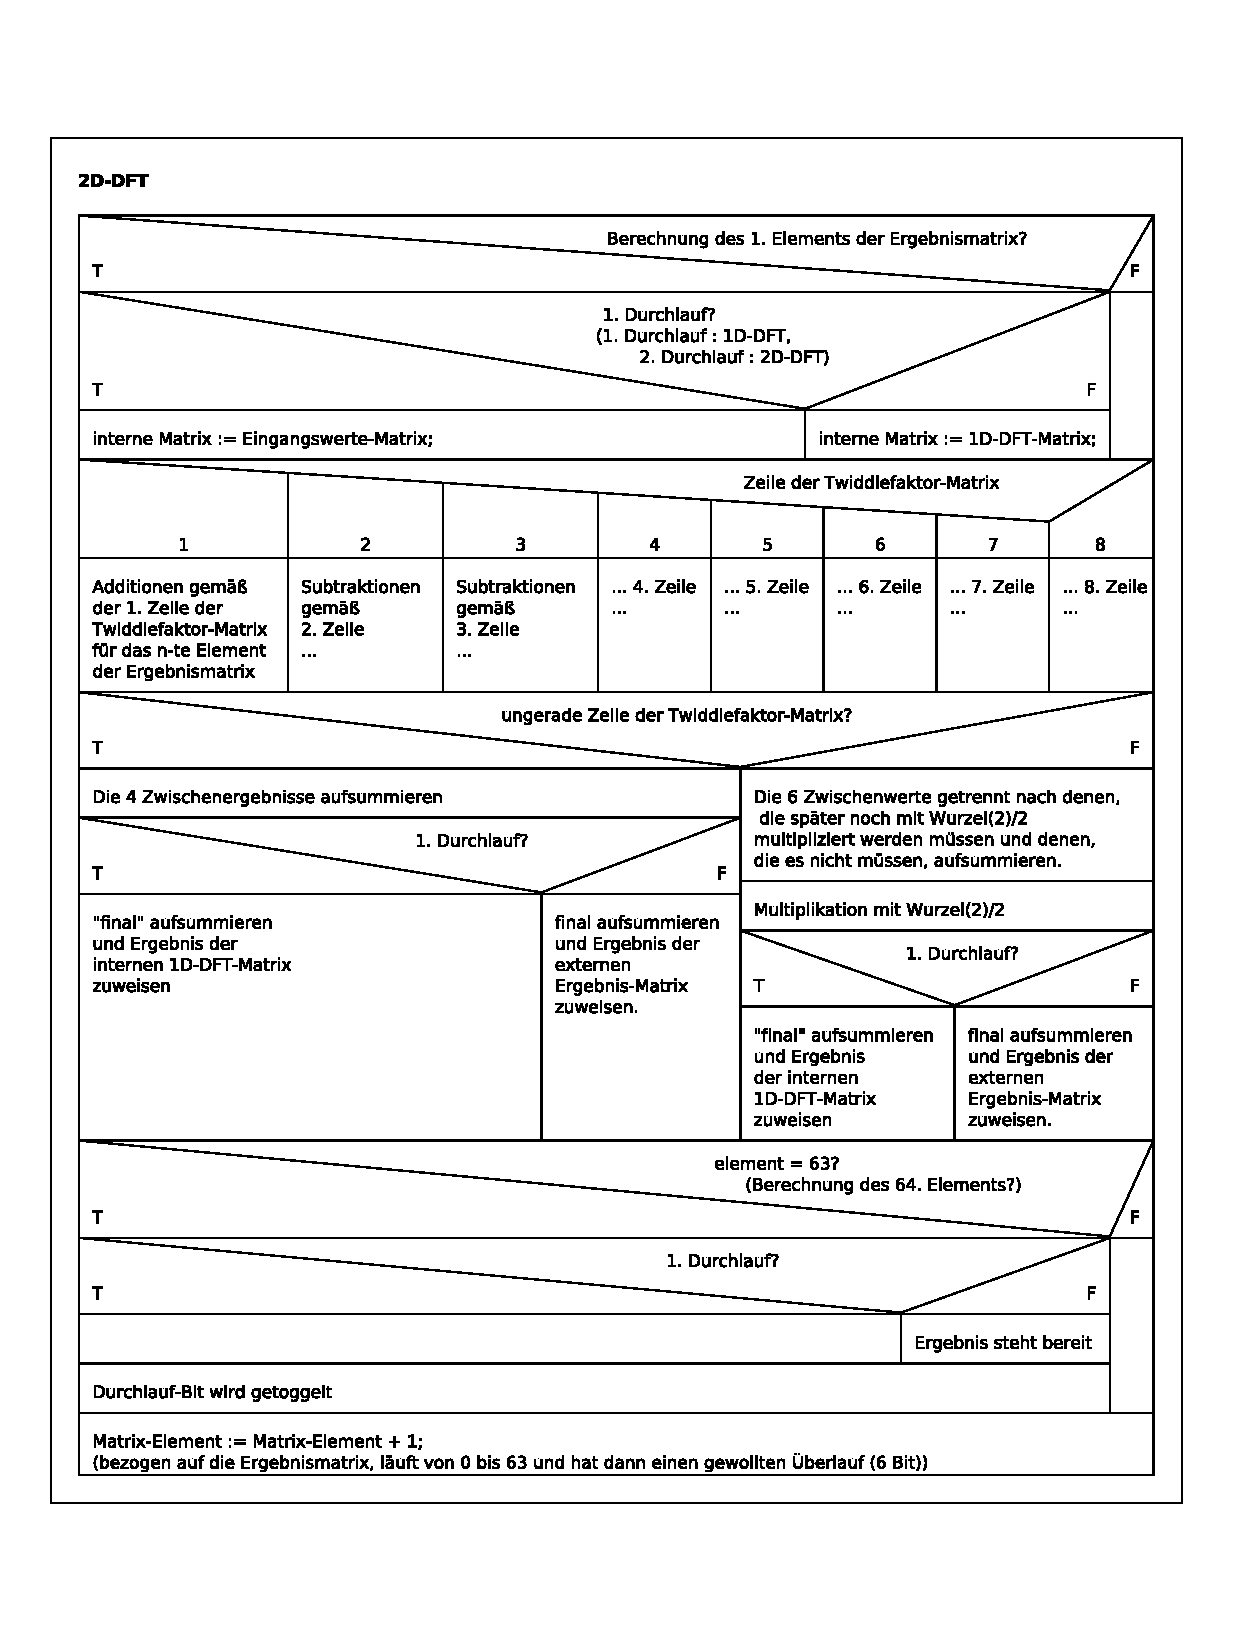
\includepdf{content/Struktogramm.pdf}

\section{Schema der Zustandsfolge}
test test

 \begin{figure}[t!]
 \centering
\begin{tikzpicture}[->,>=stealth',shorten >=1pt,auto,node distance=4.5cm,
                    semithick,initial text=nReset, initial where=above]
  \tikzstyle{every state}=[fill=white, text=black]
  %\tikzstyle{every initial where}=[above]
  

  \node[initial,state, circle split,minimum size=70pt] (A)                   {Idle};
  \node[state, circle split, minimum size=65pt]         (B) [below right of=A]{Twiddle\_Calc};
  \node[state, circle split, minimum size=65pt]         (C) [below right of=B]      {Additions\_1};
  \node[state, circle split, minimum size=65pt]         (D) [below of=C] {Additions\_2};
  \node[state, circle split, minimum size=65pt]         (E) [below left of=D] {Const\_mult};
  \node[state, circle split, minimum size=65pt]         (F) [above left of=E]      {Additions\_3};
  \node[state, circle split, minimum size=65pt]         (G) [above of=F]      {set\_ready\_bit};

  
   \path (A) edge (B) 
         (A) [loop left] edge(A)
         (B) [bend left=10] edge (C)
         (C) edge (D)
         (D) edge (B)
         (D) edge (E)
         (E) edge (F)
         (F) [bend right=10] edge (B)
         (F) [bend left=10] edge (G)
         (G) edge (B);
\end{tikzpicture}
\caption{Automatengraf}
\label{pic:Automatengraf}
\end{figure}


\section{UML-Diagramm}

% Define block styles
\tikzstyle{decision} = [diamond,                    draw, fill=blue!20, text width=6em, text badly centered, node distance=4cm, inner sep=0pt]
\tikzstyle{block} =    [rectangle, rounded corners, draw, fill=blue!20, text width=5em, text centered,       node distance=4cm, minimum height=5em, minimum width=7em]
\tikzstyle{smallblock} =    [rectangle, rounded corners, draw, fill=blue!20, text width=5em, text centered,       node distance=4cm, minimum height=2em, minimum width=3.5em]
\tikzstyle{wideblock} =    [rectangle, rounded corners, draw, fill=blue!20, text width=7em, text centered,       node distance=4cm, minimum height=5em, minimum width=7em]
\tikzstyle{verywideblock} =    [rectangle, rounded corners, draw, fill=blue!20, text width=15em, text centered,       node distance=4cm, minimum height=4em, minimum width=15em]
\tikzstyle{textblock} =    [rectangle, rounded corners, draw, fill=blue!20, text width=12em, text centered,       node distance=4cm, minimum height=4em, minimum width=10em]
\tikzstyle{dot}=[draw,shape=circle]

\tikzstyle{arrowline} = [draw, -latex']


    
\begin{tikzpicture}[auto, node distance = 1cm and 1cm, initial text=POR, initial where=above]
    % Place nodes
    \node [initial, smallblock] (start) {Idle};
    \node [decision, below of=start, node distance=3cm] (init) {IDFT?};
    \node [block, below right of=init, node distance=3cm] (Zeilenindex) {Zeilenindex tauschen};
    \coordinate[below of=init, node distance=3.5cm](Punkt_0);
    \node [decision, below of=Punkt_0, node distance=2cm] (Element_1) {Berechnung 1. Element?};
    \coordinate [right of=Element_1, node distance=4cm](c1);
    \node [decision, below of=c1, node distance=2cm] (Berechnung_1D_1) {Berechnung 1D-DFT?};
    
    \node [block, below of=Berechnung_1D_1, node distance=3cm] (überschreiben_mit_eingangswerten) {Zwischen- werte := 1D-DFT-Werten};
    \node [block, right of=überschreiben_mit_eingangswerten, node distance=4cm] (überschreiben_mit_1D_Werten) {Zwischen- werte := Eingangswerte};
    \node [block, left of=überschreiben_mit_eingangswerten, node distance=4cm] (Werte_beibehalten) {Zwischen- werte := Zwischen- werte};
    
    \node [dot, fill, inner sep=1pt, below of=überschreiben_mit_eingangswerten,node distance=1.5cm] (Punkt_1){};
    \node [decision,                 below of=Punkt_1,node distance=2cm] (Zustandsabfrage) {Zeilen- abfrage};
    
    \node [dot, fill, inner sep=1pt, below of=Zustandsabfrage,node distance=2cm] (Punkt_2){};
    \coordinate[below of=Punkt_2, node distance=0.5cm](Punkt_3);
    
    \node [textblock, right of=Punkt_2, node distance=3cm] (Zeile_1){Berechnungen entsprechend Zeile 1 der Twiddlefaktor-Matrix};
      
    \coordinate[below of=Punkt_3](Punkt_4);
    \coordinate[below of=Punkt_4,node distance=0.5cm] (Punkt_5);
    \node [textblock, right of=Punkt_5, node distance=3cm] (Zeile_8){Berechnungen entsprechend Zeile 8 der Twiddlefaktor-Matrix};
    
    \coordinate[right of=Zeile_1, node distance=3cm](Punkt_6);
    \coordinate[below of=Punkt_6, node distance=0.5cm] (Punkt_7);
    \node [dot, fill, inner sep=0.01pt, right of=Zeile_8, node distance=3cm](Punkt_9){};
    \coordinate[above of=Punkt_9, node distance=0.5cm] (Punkt_8);
    \coordinate[below of=Punkt_9, node distance=2cm](Punkt_10);
    \coordinate[left of=Punkt_10, node distance=12cm](Punkt_return_1);
    
    \coordinate[right of=init, node distance=8cm](textfeld);
    \node [draw, text, fill=white, above of=textfeld, node distance=1.3cm](tf){Zustand 2: Twiddle\_Calc};
    \coordinate[right of=start, node distance=7.1cm](textfeld2);
    \node [draw, text, fill=white, above of=textfeld2, node distance=1cm](tf2){Zustand 1: Idle};
    \node [dot, fill, inner sep=1pt, above of=init, node distance=1.7cm](Knoten_init){};
    
   % Koordinaten für Hintergrund
   \coordinate [above of=start, node distance=1.5cm](b11);
   \coordinate [right of=start, node distance=13.6cm](b12);
   \coordinate [below of=start, node distance=1cm](b13);
   \coordinate [left of=start, node distance=1.5cm](b14);
    
    % Draw edges
    \draw (start) -- (Knoten_init);
    \path [arrowline] (Knoten_init) -- (init);
    \path [arrowline] (init) -| node [near start] {ja} (Zeilenindex);
    \draw (Zeilenindex) |- (Punkt_0);    
    \draw (init) -- node [left, near start] {nein} (Punkt_0);
    \path [arrowline] (Punkt_0) -- (Element_1);
    \path [arrowline] (Element_1) -| node [near start] {ja} (Berechnung_1D_1);
    \path [arrowline] (Berechnung_1D_1) -- node [near start] {nein} (überschreiben_mit_eingangswerten);
    \path [arrowline] (Berechnung_1D_1) -| node [near start] {ja} (überschreiben_mit_1D_Werten);
    \path [arrowline] (Element_1) -- node [left, near start] {nein} (Werte_beibehalten);
    
    \draw (Werte_beibehalten) |- (Punkt_1);
    \draw (überschreiben_mit_eingangswerten) -- (Punkt_1);
    \draw (überschreiben_mit_1D_Werten) |- (Punkt_1);
    \path [arrowline] (Punkt_1) -- (Zustandsabfrage);
    \draw (Zustandsabfrage) -- (Punkt_2);
    
    \path [arrowline] (Punkt_2) -- (Zeile_1);
    \draw (Punkt_2) -- (Punkt_3);
    \draw [loosely dotted] (Punkt_3) -- (Punkt_4);
    \draw (Punkt_4) -- (Punkt_5);
    \path [arrowline](Punkt_5) -- (Zeile_8);
    
    \draw (Zeile_1) -- (Punkt_6);
    \draw (Punkt_6) -- (Punkt_7);
    \draw [loosely dotted] (Punkt_7) -- (Punkt_8);
    \draw (Punkt_8) -- (Punkt_9);
    \draw (Zeile_8) -- (Punkt_9);
    \draw (Punkt_9) -- (Punkt_10);
    \draw (Punkt_return_1) |- (Knoten_init);
    \path (start) [loop right] edge (start);
    
     \begin{pgfonlayer}{background}
      \filldraw [fill=gray!20, draw=gray!15]
        (b11.north -| b12.west)  rectangle (b13.south -| b14.east);
     \end{pgfonlayer}

    
\end{tikzpicture}

\begin{tikzpicture}[auto, node distance = 1cm and 1cm, initial text="", initial where=above]



\node [initial, decision] (gerade_Zeile_1) {gerade Zeile?};
\node [wideblock, below left of=gerade_Zeile_1] (gerade_Zeile_1_aufsummieren) {Zwischenwerte paarweise aufsummieren};
\node [wideblock, below right of=gerade_Zeile_1] (ungerade_Zeile_1_aufsummieren) {Zwischenwerte paarweise aufsummieren, zu multiplizierende getrennt};
\node [dot, fill, inner sep=1pt, below of=gerade_Zeile_1, node distance=5cm](Punkt_1){};


\node [decision, below of=Punkt_1, node distance=4cm] (gerade_Zeile_2) {gerade Zeile?};
\coordinate [left of=gerade_Zeile_2, node distance=3.5cm] (Punkt_gerade_Zeile_2);
\coordinate [right of=gerade_Zeile_2, node distance=3.5cm] (Punkt_gerade_Zeile_2_2);

\node [block, below of=Punkt_gerade_Zeile_2, node distance=3cm] (ungerade_Zeile_2_aufsummieren) {Letztes Paar aufsummieren};
\node [block, below of=Punkt_gerade_Zeile_2_2, node distance=3cm] (gerade_Zeile_2_aufsummieren) {Letztes Multiplikationspaar aufsummieren};
\node [decision, below of=ungerade_Zeile_2_aufsummieren, node distance=3cm] (Berechnung_1D_2) {Berechnung 1D-DFT?};

\node [block, below left of=Berechnung_1D_2, node distance=3.2cm] (Werte_extern_speichern_1) {Werte in (externe) 2D-DFT-Matrix speichern};
\node [block, below right of=Berechnung_1D_2, node distance=3.2cm] (Werte_intern_speichern_1) {Werte in (interne) 1D-DFT-Matrix speichern};
\coordinate [below of=Werte_extern_speichern_1, node distance=2cm](Punkt_3);
\coordinate [below of=Werte_intern_speichern_1, node distance=2cm](Punkt_4);

\coordinate (Middle_2) at ($(Punkt_3)!0.5!(Punkt_4)$);
\node [dot, fill, inner sep=1pt,  above of=Middle_2, node distance=0cm] (Middle_2_dot){};
\node [block, below of=Middle_2, node distance=1.5cm] (Matrix_Element_plus_1_1) {Matrix-Element += 1};
\coordinate [below=of Matrix_Element_plus_1_1](Punkt_5);

\coordinate [left of=Punkt_5, node distance=6cm] (Punkt_unten_links);
\node [dot, fill, inner sep=1pt, above of=Punkt_unten_links, node distance=0.5cm](Knoten_unten_links){};
\coordinate [below of=gerade_Zeile_2_aufsummieren, node distance=10.8cm] (Punkt_unten_rechts);
\coordinate [above of=Punkt_unten_links, node distance=25cm] (Punkt_oben_links);

 % Koordinaten für Hintergrund
 \coordinate [above of=gerade_Zeile_1, node distance=2.1cm](b11);
 \coordinate [right of=ungerade_Zeile_1_aufsummieren, node distance=3.3cm](b12);
 \coordinate [above of=gerade_Zeile_2, node distance=3cm](b13);
 \coordinate [left of=gerade_Zeile_1_aufsummieren, node distance=6cm](b14);
 
 % Text
 \coordinate[left of=gerade_Zeile_1, node distance=5.5cm](textfeld);
 \node [draw, text, fill=white, above of=textfeld, node distance=1.2cm](tf){Zustand 3: Summation\_1};
 
 \node [draw, text, below of=textfeld, node distance=7cm](tf2){Zustand 4: Summation\_2}; 


\path [arrowline] (gerade_Zeile_1) -| node [above, near start] {nein} (gerade_Zeile_1_aufsummieren);
\path [arrowline] (gerade_Zeile_1) -| node [near start] {ja} (ungerade_Zeile_1_aufsummieren);
\draw (gerade_Zeile_1_aufsummieren) |- (Punkt_1);
\draw (ungerade_Zeile_1_aufsummieren) |- (Punkt_1); 
\path [arrowline] (Punkt_1) -- (gerade_Zeile_2);

\draw (gerade_Zeile_2) -- node [above, near start] {nein} (Punkt_gerade_Zeile_2);
\path [arrowline] (Punkt_gerade_Zeile_2) -| (ungerade_Zeile_2_aufsummieren);
\draw (gerade_Zeile_2) -- node [near start] {ja} (Punkt_gerade_Zeile_2_2);

\path [arrowline] (Punkt_gerade_Zeile_2_2) -| (gerade_Zeile_2_aufsummieren);
\path [arrowline] (ungerade_Zeile_2_aufsummieren) -- (Berechnung_1D_2);
\path [arrowline] (Berechnung_1D_2) -| node [above] {nein} (Werte_extern_speichern_1);
\path [arrowline] (Berechnung_1D_2) -| node [above] {ja} (Werte_intern_speichern_1);
\draw (Werte_extern_speichern_1) -- (Punkt_3);
\draw (Werte_intern_speichern_1) -- (Punkt_4);
\draw (Punkt_3) -- (Middle_2);
\draw (Punkt_4) -- (Middle_2);
\path [arrowline] (Middle_2) -- (Matrix_Element_plus_1_1);
\draw (Matrix_Element_plus_1_1) |- (Knoten_unten_links);
\draw (Punkt_unten_links) -- (Knoten_unten_links);
\path [arrowline] (Knoten_unten_links) -- (Punkt_oben_links);
\path [arrowline](gerade_Zeile_2_aufsummieren) -- (Punkt_unten_rechts);

 \begin{pgfonlayer}{background}
  \filldraw [fill=gray!20, draw=gray!5]
  (b11.north -| b12.west)  rectangle (b13.south -| b14.east);
 \end{pgfonlayer}


\end{tikzpicture}


\begin{tikzpicture}[auto, node distance = 1cm and 1cm, initial text="", initial where=above]
 \node [initial, verywideblock] (Multiplikation) {Multiplikation durchführen};
 \node [verywideblock, below of=Multiplikation, node distance=2.5cm] (letzte_Summation){Additionskomponente und Multiplikationskompnente aufsummieren};
 \node [decision, below of=letzte_Summation, node distance=3cm] (Berechnung_1D_3) {Berechnung 1D-DFT?};
 \node [block, below left of=Berechnung_1D_3, node distance=3.5cm] (Werte_extern_speichern_2) {Werte in (externe) 2D-DFT-Matrix speichern};
 \node [block, below right of=Berechnung_1D_3, node distance=3.5cm] (Werte_intern_speichern_2) {Werte in (interne) 1D-DFT-Matrix speichern};
 
 \node [dot, fill, inner sep=1pt, below of=Berechnung_1D_3, node distance=4cm](Knoten_berechnung_dft2){};
 \node [decision, below of=Knoten_berechnung_dft2, node distance=2cm] (Element_63) {Berechnung 63. Element};
 
 \coordinate [left of=Element_63, node distance=3cm] (links_neben_element_63);
 \node [dot, fill, inner sep=1pt, below of=links_neben_element_63, node distance=5.5cm] (Knoten_über_matrix_element_plus1_2) {};
 \node [block, below of=Knoten_über_matrix_element_plus1_2, node distance=1.6cm] (Matrix_Element_plus_1_2){Matrix-Element += 1};
 
 \node [decision, below right of=Element_63, node distance=3cm] (Berechnung_1D_4) {Berechnung 1D-DFT?};
 \node [block, below left of=Berechnung_1D_4, node distance=3cm] (dft_1d_2d_2) {DFT\_1D\_2D := 2D};
 \node [block, below right of=Berechnung_1D_4, node distance=3cm] (dft_1d_2d_1) {DFT\_1D\_2D := 1D};
 \node [block, below of=dft_1d_2d_1, node distance=3cm] (Matrix_Element_plus_1_3){Matrix-Element += 1};
 \node [block, below of=Matrix_Element_plus_1_3, node distance=3cm] (set_ready_bit) {Ready-Bit setzen};
 \coordinate [below of=set_ready_bit, node distance=1.5cm](unter_set_ready_bit);
 \coordinate [left of=unter_set_ready_bit, node distance=14cm](Punkt_unten_links);
 \node [dot, fill, inner sep=1pt, above of=Punkt_unten_links, node distance=3cm](knoten_für_plus_1){};
 \coordinate [above of=knoten_für_plus_1, node distance=21.5cm] (Punkt_oben_links);
 
 % Koordinaten für Hintergrund
 \coordinate [above of=Multiplikation, node distance=1.3cm](b11);
 \coordinate [right of=Multiplikation, node distance=5.8cm](b12);
 \coordinate [below of=Multiplikation, node distance=1.3cm](b13);
 \coordinate [left of=Multiplikation, node distance=9cm](b14);
 
 \coordinate [above of=set_ready_bit, node distance=1.3cm](b21);
 \coordinate [right of=set_ready_bit, node distance=1.6cm](b22);
 \coordinate [below of=set_ready_bit, node distance=1.3cm](b23);
 \coordinate [left of=set_ready_bit, node distance=13.2cm](b24);
 
  % Text
 \coordinate[left of=Multiplikation, node distance=6cm](textfeld);
 \node [draw, text, fill=white, above of=textfeld, node distance=0.5cm](tf){Zustand 5: Const\_Mult};
 \node [draw, text, fill=white, below of=textfeld, node distance=2cm](tf){Zustand 6: Summation\_3};
 \node [draw, text, fill=white, below of=textfeld, node distance=21.2cm](tf){Zustand 7: Set\_Ready\_Bit};
 
 
 \path [arrowline] (Multiplikation) -- (letzte_Summation);
 \path [arrowline] (letzte_Summation) -- (Berechnung_1D_3);
 \path [arrowline] (Berechnung_1D_3) -| node [above] {nein} (Werte_extern_speichern_2);
 \path [arrowline] (Berechnung_1D_3) -| node [above] {ja} (Werte_intern_speichern_2);
 \draw (Werte_extern_speichern_2) |- (Knoten_berechnung_dft2);
 \draw (Werte_intern_speichern_2) |- (Knoten_berechnung_dft2);
 \path [arrowline] (Knoten_berechnung_dft2) -- (Element_63);
 \draw (Element_63) -- node [above] {nein} (links_neben_element_63);
 \draw (links_neben_element_63) -- (Knoten_über_matrix_element_plus1_2);
 \draw (dft_1d_2d_2) |- (Knoten_über_matrix_element_plus1_2);
 \path [arrowline] (Knoten_über_matrix_element_plus1_2) -- (Matrix_Element_plus_1_2);
 \path [arrowline] (Berechnung_1D_4) -| node [above] {ja} (dft_1d_2d_2);
 
 \path [arrowline] (Element_63) -| node [above] {ja} (Berechnung_1D_4);
 \path [arrowline] (Berechnung_1D_4) -| node [above] {nein} (dft_1d_2d_1);
 \path [arrowline] (dft_1d_2d_1) -- (Matrix_Element_plus_1_3);
 \path [arrowline] (Matrix_Element_plus_1_3) -- (set_ready_bit);
 
 \draw (set_ready_bit) -- (unter_set_ready_bit);
 \draw (unter_set_ready_bit) -- (Punkt_unten_links);
 \path [arrowline] (Punkt_unten_links) -- (Punkt_oben_links);
 \draw (Matrix_Element_plus_1_2) |- (knoten_für_plus_1);
 
 \begin{pgfonlayer}{background}
  \filldraw [fill=gray!20, draw=gray!15]
  (b11.north -| b12.west)  rectangle (b13.south -| b14.east)
  (b21.north -| b22.west)  rectangle (b23.south -| b24.east);
 \end{pgfonlayer}

 
\end{tikzpicture}

%\end{landscape}
